\documentclass[a4paper,german,12pt,smallheadings]{scrartcl}
\usepackage[T1]{fontenc}
\usepackage[utf8]{inputenc}
\usepackage{babel}
\usepackage{tikz}
\usetikzlibrary{calc,fadings,decorations.pathreplacing}
%% helper macros

\newcommand\pgfmathsinandcos[3]{%
  \pgfmathsetmacro#1{sin(#3)}%
  \pgfmathsetmacro#2{cos(#3)}%
}
\newcommand\LongitudePlane[3][current plane]{%
  \pgfmathsinandcos\sinEl\cosEl{#2} % elevation
  \pgfmathsinandcos\sint\cost{#3} % azimuth
  \tikzset{#1/.estyle={cm={\cost,\sint*\sinEl,0,\cosEl,(0,0)}}}
}
\newcommand\LatitudePlane[3][current plane]{%
  \pgfmathsinandcos\sinEl\cosEl{#2} % elevation
  \pgfmathsinandcos\sint\cost{#3} % latitude
  \pgfmathsetmacro\yshift{\cosEl*\sint}
  \tikzset{#1/.estyle={cm={\cost,0,0,\cost*\sinEl,(0,\yshift)}}} %
}
\newcommand\DrawLongitudeCircle[2][1]{
  \LongitudePlane{\angEl}{#2}
  \tikzset{current plane/.prefix style={scale=#1}}
   % angle of "visibility"
  \pgfmathsetmacro\angVis{atan(sin(#2)*cos(\angEl)/sin(\angEl))} %
  \draw[current plane] (\angVis:1) arc (\angVis:\angVis+180:1);
  \draw[current plane,dashed] (\angVis-180:1) arc (\angVis-180:\angVis:1);
}
\newcommand\DrawLatitudeCircle[2][1]{
  \LatitudePlane{\angEl}{#2}
  \tikzset{current plane/.prefix style={scale=#1}}
  \pgfmathsetmacro\sinVis{sin(#2)/cos(#2)*sin(\angEl)/cos(\angEl)}
  % angle of "visibility"
  \pgfmathsetmacro\angVis{asin(min(1,max(\sinVis,-1)))}
  \draw[current plane] (\angVis:1) arc (\angVis:-\angVis-180:1);
  \draw[current plane,dashed] (180-\angVis:1) arc (180-\angVis:\angVis:1);
}

%% document-wide tikz options and styles

\tikzset{%
  >=latex, % option for nice arrows
  inner sep=0pt,%
  outer sep=2pt,%
  mark coordinate/.style={inner sep=0pt,outer sep=0pt,minimum size=3pt,
    fill=black,circle}%
}

\usepackage{geometry}
\usepackage{amsmath}
\usepackage{amssymb}
\usepackage{float}
\usepackage{enumerate}
\usepackage{braket} % Teh quantum stuff
\usepackage{commath} % http://tex.stackexchange.com/questions/14821/whats-the-proper-way-to-typeset-a-differential-operator
\usepackage{cancel}
%\usepackage{wrapfig}
\usepackage[thinspace,thinqspace,squaren,textstyle]{SIunits}

% New command for color underlining
\usepackage{xcolor}

\newsavebox\MBox
\newcommand\colul[2][red]{{\sbox\MBox{$#2$}%
  \rlap{\usebox\MBox}\color{#1}\rule[-1.2\dp\MBox]{\wd\MBox}{0.5pt}}}

\restylefloat{table}
\geometry{a4paper, top=15mm, left=20mm, right=40mm, bottom=20mm, headsep=10mm, footskip=12mm}
\linespread{1.5}
\setlength\parindent{0pt}
\DeclareMathOperator{\Tr}{Tr}
\begin{document}
\allowdisplaybreaks % Seitenumbrüche in Formeln erlauben
\begin{center}
\bfseries % Fettdruck einschalten
\sffamily % Serifenlose Schrift
\vspace{-40pt}
Quantum Mechanics, winter term 2013/2014, exercise sheet 6

Markus Fenske, Tutor: Adam Nagy
\vspace{-10pt}
\end{center}

\section*{Exercise 1: spin $1/2$ particle in magnetic field}
\begin{enumerate}[a)]
  \item
    Using
    \begin{equation*}
    \sigma_x = \begin{pmatrix}0 & 1 \\ 1 & 0\end{pmatrix} \qquad \sigma_z = \begin{pmatrix}1 & 0 \\ 0 & -1\end{pmatrix}
    \end{equation*}

    We get
    \begin{equation*}
    H = B \begin{pmatrix} \cos \theta & \sin \theta \\ \sin \theta & -\cos \theta \end{pmatrix}
    \end{equation*}

    The eigenvalues of the matrix dived by $B$ are
    \begin{align*}
    &B \begin{vmatrix} \cos(\theta) - \lambda & \sin \theta \\ \sin \theta & -\cos(\theta) - \lambda \end{vmatrix} \overset{!}{=} 0 \\
      \Leftrightarrow\quad&B \del{-\del{\cos\del{\theta} - \lambda}^2-\sin^2\del{\theta}}  = 0\\
      \Leftrightarrow\quad&B \del{-\cos^2\del\theta \cancel{-\lambda\cos\del\theta}\cancel{+\lambda\cos\del\theta}+\lambda^2-\sin^2\del\theta} = 0\\
      \Leftrightarrow\quad&B \del{-\cancelto{1}{\del{\cos^2\del\theta+\sin^2\del\theta}}+\lambda^2} = 0\\
      \Leftrightarrow\quad&B \del{-1+\lambda^2} = 0\\
      \Rightarrow\quad &\lambda_+ = 1,\quad \lambda_- = -1
    \end{align*}

    Because we divided by $B$, the eigenvalues are
    \begin{equation*}
      \lambda_+ = B,\quad \lambda_- = -B
    \end{equation*}

    Calculatring the eigenvectors (assuming $\sin\theta \neq 0$)
    \begin{align*}
      &\begin{pmatrix}
        \cos\del\theta - \lambda_\pm & \sin \theta \\
        \sin\theta & -\cos\del\theta - \lambda_\pm \\
      \end{pmatrix}
      &\xrightarrow[\text{leading elements}]{\text{Crossdivide by}}&
      \begin{pmatrix}
        1 & \frac{\sin \theta}{\cos\del\theta-\lambda_\pm} \\
        1 & \frac{-\cos\del\theta - \lambda_\pm}{\sin\theta} \\
      \end{pmatrix}
      &\xrightarrow[\text{I from II}]{\text{Subtract}} \\
      &\begin{pmatrix}
        1 & \frac{\sin \theta}{\cos\del\theta-\lambda_\pm} \\
        0 & \frac{-\cos\del\theta - \lambda_\pm}{\sin\theta} - \frac{\sin \theta}{\cos\del\theta-\lambda_\pm} \\
      \end{pmatrix}
      &=&
      \begin{pmatrix}
        1 & \frac{\sin \theta}{\cos\del\theta-\lambda_\pm} \\
        0 & \frac{-\del{\cos\del\theta - \lambda_\pm}^2 - \sin^2\del\theta}{\sin\theta\del{\cos\del\theta-\lambda_\pm}} \\
      \end{pmatrix}
      &= \\
      &\begin{pmatrix}
        1 & \frac{\sin \theta}{\cos\del\theta-\lambda_\pm} \\
        0 & \frac{-\cos^2\theta\cancel{+\cos\theta}\cancel{-\cos\theta}+1-\sin^2\theta}{\sin\theta\del{\cos\del\theta-\lambda_\pm}} \\
      \end{pmatrix}
      &=&
      \begin{pmatrix}
        1 & \frac{\sin \theta}{\cos\del\theta-\lambda_\pm} \\
        0 & \frac{-\del{\cos^2\theta+\sin^2\theta}+1}{\sin\theta\del{\cos\del\theta-\lambda_\pm}} \\
      \end{pmatrix}
      &= \\
      &\begin{pmatrix}
        1 & \frac{\sin \theta}{\cos\del\theta-\lambda_\pm} \\
        0 & 0 \\
      \end{pmatrix}
      &\xrightarrow[x_1 = 1]{\text{Choose}}&
      \quad x_2 = \frac{\sin\theta}{\cos\del\theta - \lambda_\pm}
    \end{align*}

    So the eigenvectors are (by multiplying with $\cos\del\delta \mp 1$):
    \begin{equation*}
    \ket{\psi_\pm} = \begin{pmatrix} \cos\del\theta \mp 1 \\ \sin\theta \end{pmatrix}
    \end{equation*}

    I can now prove, that the projections cannot be written as the matrix given
    on the exercise sheet. For projections, we must demand that
    \begin{align*}
      A = \sum_i \lambda_i \ket{\psi_i}\bra{\psi_i}
    \end{align*}
    where $\lambda_i$ are the eigenvalues, $\psi_i$ are the eigenvevtors and
    $A$ is the original operator. So in this case, it must be true that

    \begin{equation*}
      \lambda_+ \ket{\psi_+} \bra{\psi_+} + \lambda_- \ket{\psi_-} \bra{\psi_-} = H
    \end{equation*}

    Using the given projections
    \begin{equation*}
      \ket{\psi_\pm} \bra{\psi_\pm} = \frac{1}{2} \begin{pmatrix}
        1 \mp \cos \theta & \pm \sin \theta \\
        \pm \sin \theta & 1 \pm \cos \theta
      \end{pmatrix}
    \end{equation*}

    We get
    \begin{align*}
      \lambda_+ \ket{\psi_+} \bra{\psi_+} + \lambda_- \ket{\psi_-} \bra{\psi_-} &=
      \frac{1}{2} \begin{pmatrix}
        1 - \cos \theta &  \sin \theta \\
         \sin \theta & 1 + \cos \theta
      \end{pmatrix}
      +
      \frac{1}{2} \begin{pmatrix}
        1 + \cos \theta &  -\sin \theta \\
         -\sin \theta & 1 - \cos \theta
      \end{pmatrix}\\
      &=
      \begin{pmatrix}
        -\cos \theta &  \sin \theta \\
         \sin \theta &  \cos \theta
      \end{pmatrix}
      \neq
      \begin{pmatrix}
        \cos \theta &  \sin \theta \\
         \sin \theta &  -\cos \theta
      \end{pmatrix}
    \end{align*}

    So the given projections are wrong. The correct projections would be
    \begin{equation*}
      \ket{\psi_\pm} \bra{\psi_\pm} = \frac{1}{2} \begin{pmatrix}
        1 \pm \cos \theta & \pm \sin \theta \\
        \pm \sin \theta & 1 \mp \cos \theta
      \end{pmatrix}
    \end{equation*}
  \item
    Using the correct projections, we can now calculate the matrix exponential.
    As proven in the last exercise sheet, we just need to calculate the
    exponential of the eigenvalues, as the projects are idempontent ($P^2 =
    P$).
    \begin{align*}
      \exp\del{\frac{-itH}{\hbar}} &= \exp\del{\lambda_+} \ket{\psi_+}\bra{\psi_+} + \exp\del{\lambda_-} \ket{\psi_-}\bra{\psi_-} \\
                                   &= 
      \begin{pmatrix}
        \frac{\cos(\theta) + 1}{2} \exp\del{-B\frac{it}{\hbar}} + \frac{\cos(\theta) - 1}{2} \exp\del{B\frac{it}{\hbar}} &
        \frac{\sin\theta}{2} \exp\del{-B\frac{it}{\hbar}} - \frac{\sin\theta}{2} \exp\del{B\frac{it}{\hbar}} \\
        \frac{\sin\theta}{2} \exp\del{-B\frac{it}{\hbar}} - \frac{\sin\theta}{2} \exp\del{B\frac{it}{\hbar}} &
        \frac{\cos(\theta) - 1}{2} \exp\del{-B\frac{it}{\hbar}} + \frac{\cos(\theta) + 1}{2} \exp\del{B\frac{it}{\hbar}}
      \end{pmatrix}
    \end{align*}
  \item
    We know that
    \begin{equation*}
      \ket{\psi(t)} = U(t,t_0) \ket{\psi(t_0)}
    \end{equation*}

    So
    \begin{align*}
      \ket{\psi(t)} &= U_t \ket{0} \\
                    &= 
      \begin{pmatrix}
        \frac{\cos(\theta) + 1}{2} \exp\del{-B\frac{it}{\hbar}} + \frac{\cos(\theta) - 1}{2} \exp\del{B\frac{it}{\hbar}} \\
        \frac{\sin\theta}{2} \exp\del{-B\frac{it}{\hbar}} - \frac{\sin\theta}{2} \exp\del{B\frac{it}{\hbar}}
      \end{pmatrix}
    \end{align*}
  \item
    The probability is
    \begin{align*}
      p &= \envert{\braket{\psi(t)|1}}^2 \\
        &=  \envert{\frac{\sin\theta}{2} \exp\del{-B\frac{it}{\hbar}} - \frac{\sin\theta}{2} \exp\del{B\frac{it}{\hbar}}}^2 \\
        &=  \envert{i\sin\del\theta\sin\del{-B\frac{t}{\hbar}}}^2 \\
        &=  \sin^2\del\theta\sin^2\del{-B\frac{t}{\hbar}}
    \end{align*}

  \item
    For $\theta = \frac{\pi}{4}$ we get
    \begin{align*}
      \ket{\psi(t)} &= 
      \begin{pmatrix}
        \frac{\frac{1}{\sqrt{2}} + 1}{2} \exp\del{-B\frac{it}{\hbar}} + \frac{\frac{1}{\sqrt{2}} - 1}{2} \exp\del{B\frac{it}{\hbar}} \\
        \frac{1}{2\sqrt{2}} \exp\del{-B\frac{it}{\hbar}} - \frac{1}{2\sqrt{2}} \exp\del{B\frac{it}{\hbar}}
      \end{pmatrix} \\
      &= 
      \begin{pmatrix}
        \frac{\frac{1}{\sqrt{2}} + 1}{2} \exp\del{-B\frac{it}{\hbar}} + \frac{\frac{1}{\sqrt{2}} - 1}{2} \exp\del{B\frac{it}{\hbar}} \\
        \frac{i}{\sqrt{2}} \sin  \frac{Bt}{\hbar}
      \end{pmatrix}
    \end{align*}

    So we can now calculate some states, where $t' = \frac{Bt}{\hbar} \in [0, 2\pi]$

    \begin{align*}
      t' = 0 \Rightarrow             &\ket{0} \\
      t' = \frac{\pi}{2} \Rightarrow &-\frac{1}{\sqrt{2}}\del{\ket{0} + \ket{1}} \\
      t' = \pi \Rightarrow &-\ket{0} \\
      t' = \frac{3\pi}{2} \Rightarrow &\frac{1}{\sqrt{2}}\del{i\ket{0} + i\ket{1}} \\
    \end{align*}

    The last two states are identical to the first two.



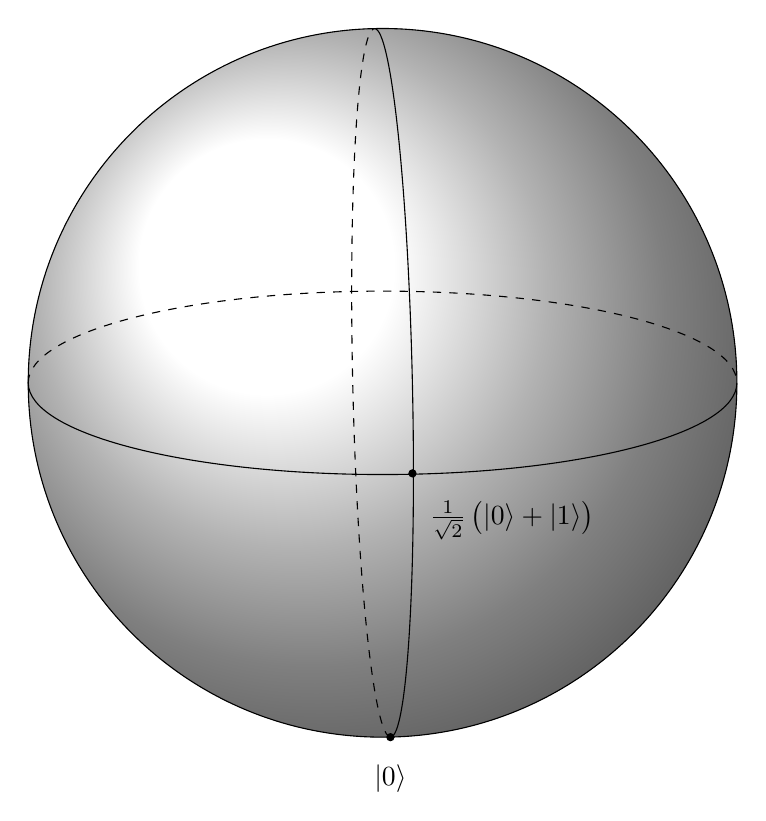
\begin{tikzpicture} % "THE GLOBE"
\def\R{4.5} % sphere radius
\def\angEl{15} % elevation angle
\filldraw[ball color=white] (0,0) circle (\R);
%\foreach \t in {-80,-60,...,80} { \DrawLatitudeCircle[\R]{\t} }
%\foreach \t in {-5,-35,...,-175} { \DrawLongitudeCircle[\R]{\t} }
\DrawLatitudeCircle[\R]{0} % equator
\DrawLongitudeCircle[\R]{95} % "nullmeridian"

\coordinate[mark coordinate] (S) at (0.1,-\R);
\coordinate[mark coordinate] (X) at (0.38,-1.15);

\node[below=8pt] at (S) {$\ket{0}$};
\node[right=36pt,below=8pt] at (X) {$\frac{1}{\sqrt{2}} \del{\ket{0} + \ket{1}}$};
\end{tikzpicture}

The states oscillate between $\ket{0}$ and $\frac{1}{\sqrt{2}} \del{\ket{0} + \ket{1}}$.



\end{enumerate}
\section*{Exercise 2: Time dependence in a box}
\begin{enumerate}[a)]
  \item
    Iff $m \neq n$
    \begin{align*}
      \braket{\psi_m|\psi_n} &= \int_0^1 \sin\del{m \pi x} \sin\del{n \pi x} \dif x \\
                             &= \int_0^1 \frac{1}{2} \del{\cos\del{\del{m-n}\pi x} - \cos\del{\del{m+n}\pi x}} \dif x \\
                             &= \frac{1}{2} \sbr{\frac{\sin\del{\del{m-n}\pi x}}{\del{m-n} \pi}}_0^1
                                - \frac{1}{2} \sbr{\frac{\sin\del{\del{m+n}\pi x}}{\del{m+n} \pi}}_0^1 \\
                             &= \frac{1}{2} \frac{\sin\del{\del{m-n}\pi}}{\del{m-n} \pi}
                                - \frac{1}{2} \frac{\sin\del{\del{m+n}\pi x}}{\del{m+n} \pi} \\
                             &= 0 \qquad\qquad \text{(Because $\sin n \pi = 0, n \in \mathbb{N}$)}
    \end{align*}
    Therefore the vectors are orthogonal.

    Iff $m = n$
    \begin{align*}
      \braket{\psi_m|\psi_n} &= \int_0^1 C^2 \sin^2\del{n \pi x} \dif x \\
                             &= \int_0^1 C^2 \frac{1}{2}\del{1 - \cos\del{2n \pi x}} \dif x \\
                             &= \frac{1}{2}C^2 - C^2 \frac{\sin\del{2n \pi}}{2n} \\
                             &= \frac{1}{2}C^2 \overset{!}{=} 0
    \end{align*}

    Therefore $C = \sqrt{2}$.
  \item
    We are looking for stationary solutions to the Schr"odinger equation.
    \begin{align*}
      \hat H\ket{\psi_n} = E\ket{\psi_n}
    \end{align*}

    We get
    \begin{align*}
      \hat H\ket{\psi_n} &= \del{\frac{1}{2m} \hat{p}^2 + V\del{\hat{x}}} \sin\del{n \pi x} \\
                         &= \del{\frac{1}{2m} \del{-i\hbar \pd{}{x}}^2 + C} \sin\del{n \pi x} \\
                         &= \del{-\frac{1}{2m} \hbar^2 \pd[2]{}{x} + C} \sin\del{n \pi x} \\
                         &= \frac{1}{2m} \hbar^2 n^2\pi^2 \sin\del{n \pi x} + C \sin\del{n \pi x} \\
                         &= \underbrace{\del{\frac{\hbar^2 n^2 \pi^2}{2m} + C}}_{=E} \sin\del{n \pi x} \\
                         &= E \ket{\psi}
    \end{align*}

    We can see, that the eigenvalues of the Hamilton operator are
    \begin{equation*}
      E = \frac{\hbar^2 n^2 \pi^2}{2m} + C
    \end{equation*}

  \item
    The Hamilton operator is time independent, therefore

    \begin{align*}
      \ket{\psi(t)} &= U(t,0) \ket{\psi(0)} \\
                    &= \frac{1}{\sqrt{2}} U(t,0) \del{\ket{\psi_0} + \ket{\psi_1}} \\
                    &= \frac{1}{\sqrt{2}} \del{\exp\del{\frac{itH}{\hbar}} \ket{\psi_0} + \exp\del{\frac{itH}{\hbar}} \ket{\psi_1}} \\
      \intertext{Using the eigenvalues of $\ket{\psi_0}$ and $\ket{\psi_1}$ (computed by the formula above), we get}
      &= \frac{1}{\sqrt{2}} \del{\exp\del{\frac{it}{\hbar} C} \ket{\psi_0} + \exp\del{\frac{it}{\hbar} \del{\frac{\hbar^2 \pi^2}{2m} + C}} \ket{\psi_1}} \\
      &= \frac{1}{\sqrt{2}} \del{\exp\del{\frac{it}{\hbar} C} + \exp\del{\frac{it}{\hbar} \del{\frac{\hbar^2 \pi^2}{2m} + C}} \sin\del{\pi x}} \\
      &= \frac{1}{\sqrt{2}} \exp\del{\frac{it}{\hbar} C} \del{1 + \exp\del{\frac{it}{\hbar} \frac{\hbar^2 \pi^2}{2m}} \sin\del{\pi x}} \\
    \end{align*}

    The expected value is
    \begin{align*}
      \braket{x}(t) &= \int_{0}^{1} \psi(t)^* x \psi(t) \dif x \\
                    &= \int_{0}^{1}
      \cancelto{\frac{1}{2}}{\frac{1}{\sqrt{2}}} \cancel{\exp\del{\frac{-it}{\hbar} C}} \del{1 + \exp\del{\frac{-it}{\hbar} \frac{\hbar^2 \pi^2}{2m}} \sin\del{\pi x}}
                       x \\
                       &\cancel{\frac{1}{\sqrt{2}}} \cancel{\exp\del{\frac{it}{\hbar} C}} \del{1 + \exp\del{\frac{it}{\hbar} \frac{\hbar^2 \pi^2}{2m}} \sin\del{\pi x}}
                        \dif x \\
                    &=
                       \int_0^1 \frac{x}{2} \del{1 + \exp\del{\frac{-it}{\hbar} \frac{\hbar^2 \pi^2}{2m}} \sin\del{\pi x}} \dif x
                       \del{1 + \exp\del{\frac{it}{\hbar} \frac{\hbar^2 \pi^2}{2m}} \sin\del{\pi x}} \\
                       &= \int_0^1 \frac{x}{2}\del{1 + 2\cos\del{\frac{-t \hbar \pi^2}{2m}} + \sin^2\del{\pi x}} \dif x \\
                       &= \frac{1}{4} + \cos\del{\frac{-t \hbar \pi^2}{2m}} \int_0^1 x \sin\del{\pi x} \dif x + \int_0^1 \frac{x}{2} \sin^2\del{\pi x} \dif x\\
                       &= \frac{1}{4} + \cos\del{\frac{-t \hbar \pi^2}{2m}} \int_0^1 x \sin\del{\pi x} \dif x + \frac{1}{2} \int_0^1 x \sin^2\del{\pi x} \dif x\\
    \end{align*}

    Solving the first integral:
    \begin{align*}
      \int_0^1 x \sin\del{\pi x} \dif x  &= \sbr{-\frac{x\cos\del{\pi x}}{\pi}}_0^1 + \frac{1}{\pi} \int_0^1 \cos\del{\pi x} \\
                                         &= \frac{1}{\pi} + 0
    \end{align*}

    Solving the second integral:
    \begin{align*}
      \int_0^1 x \sin^2\del{\pi x} \dif x  &= \int_0^1 x \frac{1}{2} \del{1- \cos\del{2 \pi x}} \dif x \\
                                           &= \frac{1}{4} + \frac{1}{2} \int_0^1 x \cos\del{2 \pi x} \\
                                           &= \frac{1}{4} + \sbr{x \frac{\sin\del{2 \pi x}}{2 \pi}}_0^1 - \int_0^1 \frac{\sin\del{2 \pi x}}{2 \pi} \dif x \\
                                           &= \frac{1}{4}
    \end{align*}

    Leads to:
    \begin{align*}
      \braket{x}(t) &= \frac{1}{4} + \cos\del{\frac{-t \hbar \pi^2}{2m}} \frac{1}{\pi} + \frac{1}{2} \cdot \frac{1}{4} \\
                    &= \frac{3}{8} + \frac{1}{\pi} \cos\del{\frac{-t \hbar \pi^2}{2m}}
    \end{align*}
  \item
    The probability is highest, when the expected value is lowest. This is the
    case if $\cos$ has the lowest value of $-1$ which is when the argument a an
    odd multiple of $\pi$.

    \begin{align*}
      &\frac{-t \hbar \pi^2}{2m} \overset{!}{=} \del{2n + 1} \pi \\
      \Leftrightarrow\quad
      &\frac{-t \hbar \pi}{2m} = 2n + 1 \\
      \Leftrightarrow\quad
      &-t = \frac{\del{2n + 1}2m}{\hbar \pi} \\
      \Leftrightarrow\quad
      &t = \frac{\del{1-2n}2m}{\hbar \pi}, n \in \mathbb{N} \\
    \end{align*}




\end{enumerate}

\section*{Exercise 3: Tensor product}
\begin{enumerate}[a)]
  \item
    \begin{equation*}
      d^2
    \end{equation*}
  \item
    \begin{align*}
      \ket{\psi} \otimes \del{\ket{\phi} + \ket{\xi}} &= \sum_{ij=1}^d \braket{i|\psi} \bra{j} \del{\ket\phi + \ket\xi} \ket{ij} \\
      &= \sum_{ij=1}^d \braket{i|\psi} \braket{j|\phi}\ket{ij} + \braket{i|\psi} \braket{j|\xi} \ket{ij} \\
      &= \sum_{ij=1}^d \braket{i|\psi} \braket{j|\phi}\ket{ij} + \sum_{ij=1}^d \braket{i|\psi} \braket{j|\xi} \ket{ij} \\
      &= \ket\psi \otimes \ket\phi + \ket\psi \otimes \ket\xi
    \end{align*}
\end{enumerate}
\end{document}
